\documentclass[conference]{IEEEtran}
\usepackage{amsmath,booktabs,graphicx,tabularx,listings,xcolor,tikz}
\usetikzlibrary{arrows.meta,positioning}
\definecolor{codebg}{RGB}{245,247,249}
\lstset{language=Python,basicstyle=\ttfamily\footnotesize,breaklines=true,backgroundcolor=\color{codebg},frame=single,columns=fullflexible,showstringspaces=false}
\begin{document}
\title{Discrete-Event Simulation and Scheduling Optimization of the MUET Point Bus System}
\author{\IEEEauthorblockN{Simulation \& Modelling -- Problem Based Learning}
\IEEEauthorblockA{Department of Software Engineering, Mehran University of Engineering and Technology, Jamshoro\\8th Semester (22SW II \& III) \quad Instructor: Engr. Umar Farooq}}
\maketitle
\begin{abstract}
The MUET Point transport system experiences long queues, overcrowding and scheduling difficulties during peak hours. This study develops a discrete-event simulation (DES) of two terminal queues and a shared bus fleet to compare fixed-timetable dispatch with a demand-responsive policy. Forty paired replications are performed for each morning and afternoon peak under normal demand, increased demand and traffic delays. With illustrative input parameters, the adaptive policy reduces mean waiting time in the normal afternoon case from 13.69 to 5.35 minutes and increases peak fleet utilization from 52.7\% to 75.6\%. The model also reveals a trade-off between service frequency and passenger occupancy. The results support controlled trials of demand-responsive dispatch without buying additional buses; they do not represent measured MUET operations.
\end{abstract}
\begin{IEEEkeywords}
discrete-event simulation, queue management, public transport, adaptive dispatch, fleet utilization
\end{IEEEkeywords}
\section{Problem identification}
MUET operates dedicated Points for students, faculty and staff travelling between Jamshoro and Hyderabad. The PBL brief identifies the STC and Main Gate terminals, morning (8:00--9:00 AM) and afternoon (2:00--3:30 PM) peaks, long passenger waits, overcrowding and static schedules that cannot react to demand or traffic \cite{brief}. The objective is to reduce waiting and congestion and improve use of the existing fleet, without arbitrary fleet expansion.

\subsection{Requirements and constraints}
\begin{itemize}
\item Students need timely, fair and safe boarding; drivers require feasible trips and breaks; administrators need efficient use of buses and predictable service.
\item Capacity limits must be respected. A bus cannot depart while already occupied on another trip. Passengers not boarded remain in their queue.
\item The comparison must use the same fleet, demand and traffic assumptions. Dispatch cannot assume a bus is available when it has not returned.
\item Operational deployment must respect actual route compatibility, terminal access, driver availability and safe loading limits.
\end{itemize}
\section{Conceptual model and assumptions}
The model represents two first-come, first-served (FCFS) queues served in batches by a shared pool of buses. Each bus alternates between available and on-trip states. A trip includes loading, travel and return/repositioning to the dispatch pool. Each passenger leaves the queue at boarding. Morning and afternoon are modeled as independent demand windows with initially empty queues and all buses available; arrival generation ends at the peak boundary, but waiting passengers are served until the queues empty.

The assignment does not provide passenger counts, capacities, fleet size, route durations or the actual timetable. Table~\ref{tab:inputs} contains explicitly assumed inputs for a reproducible experiment. In particular, the morning terminal demand is an abstract queue representation, not a claim that all inbound passengers board at campus.
\begin{table}[h]
\caption{Illustrative simulation parameters}\label{tab:inputs}
\centering\footnotesize
\begin{tabularx}{\columnwidth}{@{}lX@{}}\toprule
Parameter & Assumed value\\\midrule
Fleet and capacity & 6 buses, 40 passengers per bus\\
Peak duration & Morning: 60 min; afternoon: 90 min\\
Morning arrival rates & STC: 2.2; Main Gate: 1.5 passengers/min\\
Afternoon arrival rates & STC: 3.2; Main Gate: 1.9 passengers/min\\
Interarrival time & Exponential distribution\\
Round-trip time & Triangular (24, 30, 36) min: min, mode, max\\
Fixed headway & 15 min per terminal; 7.5 min offset\\
Adaptive trigger & 30 waiting or oldest wait reaches 10 min\\
Replications & 40 per scenario and policy\\\bottomrule
\end{tabularx}
\end{table}
\subsection{State transitions}
\begin{figure}[h]
\centering
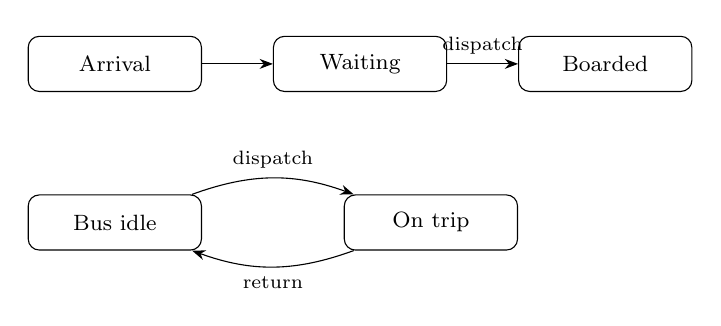
\begin{tikzpicture}[node distance=9mm, every node/.style={font=\footnotesize}, state/.style={draw,rounded corners,minimum width=22mm,minimum height=7mm,align=center}, >=Stealth]
\node[state] (a) {Arrival}; \node[state,right=of a] (q) {Waiting}; \node[state,right=of q] (b) {Boarded};
\draw[->] (a)--(q); \draw[->] (q)--node[above,font=\scriptsize]{dispatch}(b);
\node[state,below=13mm of a] (i) {Bus idle}; \node[state,right=18mm of i] (t) {On trip};
\draw[->] (i) to[bend left=20] node[above,font=\scriptsize]{dispatch} (t);
\draw[->] (t) to[bend left=20] node[below,font=\scriptsize]{return} (i);
\end{tikzpicture}
\caption{Passenger and bus state-transition diagrams.}
\end{figure}
\section{Mathematical model}
For terminal $i$, passenger interarrival time follows an exponential distribution with rate $\lambda_i$:
\begin{equation} T_i=-\frac{\ln(1-U)}{\lambda_i},\quad U\sim\mathrm{Uniform}(0,1).\end{equation}
Round-trip time $S$ follows a triangular distribution with minimum 24, mode 30 and maximum 36 minutes, so $E[S]=30$ min. For $B=6$ buses and capacity $C=40$, the ideal full-load throughput is
\begin{equation} \mu_{\max}=\frac{BC}{E[S]}=8\text{ passengers/min}.\end{equation}
This is a theoretical capacity bound, not a guaranteed throughput. The fixed schedule offers at most $2C/15=5.33$ passengers/min before missed slots and empty seats. The normal afternoon demand is $5.1$ passengers/min; high demand raises it to $6.63$, exceeding that scheduled rate. Traffic delays raise mean trip time to 42 min, reducing the ideal fleet capacity to $5.71$ passengers/min.

The batch size at departure is $b_i=\min(C,Q_i)$, with $Q_i$ the waiting queue. The queue decreases by $b_i$ and the number of idle buses decreases by one. A return event increases the idle count. For passenger $j$, $W_j=d_j-a_j$, where $a_j$ and $d_j$ are arrival and boarding times.
\begin{align}
\bar W&=\frac{1}{N}\sum_{j=1}^{N}W_j,\\
\bar Q&=\frac{1}{H}\int_0^H (Q_1(t)+Q_2(t))\,dt,\\
U_f&=\frac{100}{BH}\int_0^H B_{\rm busy}(t)\,dt,\\
L&=\frac{100N}{C D}.
\end{align}
Here $H$ is peak length, $N$ is passengers boarded after draining the queues, and $D$ is the total number of departures. $U_f$ measures bus time occupied during the peak, while $L$ measures average seat occupancy over all dispatched trips. The 95th percentile wait (P95), maximum combined queue and end-of-peak backlog are also evaluated.
\section{Simulation and scheduling algorithms}
The Python implementation uses a priority queue (\texttt{heapq}) as the future-event calendar. The clock jumps directly to the earliest event instead of advancing in fixed time increments. Arrivals, returns, dispatch slots, wait deadlines and peak snapshots are distinct events. The queue area and busy-bus area are accumulated over each interval between events.
\begin{figure}[h]
\centering
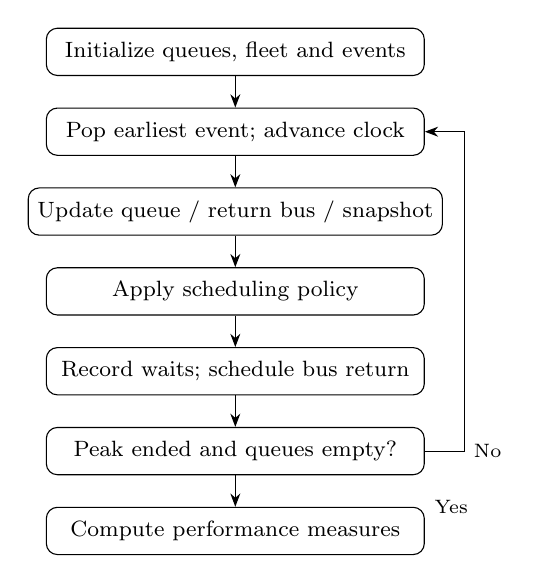
\begin{tikzpicture}[node distance=4mm, >=Stealth, every node/.style={font=\footnotesize}, flowbox/.style={draw,rounded corners,align=center,minimum width=48mm,minimum height=6mm}]
\node[flowbox] (a) {Initialize queues, fleet and events};
\node[flowbox,below=of a] (b) {Pop earliest event; advance clock};
\node[flowbox,below=of b] (c) {Update queue / return bus / snapshot};
\node[flowbox,below=of c] (d) {Apply scheduling policy};
\node[flowbox,below=of d] (e) {Record waits; schedule bus return};
\node[flowbox,below=of e] (f) {Peak ended and queues empty?};
\node[flowbox,below=of f] (g) {Compute performance measures};
\foreach \x/\y in {a/b,b/c,c/d,d/e,e/f,f/g} \draw[->] (\x)--(\y);
\draw[->] (f.east)--++(5mm,0) node[right,font=\scriptsize]{No} |- (b.east);
\node[right,font=\scriptsize] at (g.north east) {Yes};
\end{tikzpicture}
\caption{Discrete-event simulation flowchart.}
\end{figure}
\subsection{Baseline: fixed scheduling}
STC departures are attempted at minutes 0, 15, 30 and so on. Main Gate departures are attempted at minutes 7.5, 22.5, 37.5 and so on. A slot is skipped if no bus or no passenger is available. This represents a simplified static timetable, not an observed MUET schedule.
\subsection{Proposed: adaptive scheduling}
Whenever an arrival, bus return or wait-deadline event occurs, the controller checks whether an idle bus exists. A terminal qualifies when 30 passengers are waiting or its oldest passenger has waited at least 10 minutes. If both qualify, the longest-waiting terminal is selected, with queue length as the tie-breaker. After the peak, the threshold is lifted to clear outstanding queues. The 10-minute trigger is not a guaranteed maximum wait when all buses are busy.
\begin{lstlisting}[caption={Core demand-responsive dispatch rule}]
def adaptive():
    while idle:
        eligible = [i for i, q in enumerate(queues) if q and
                    (len(q) >= 30 or now - q[0] >= 10 - 1e-9 or now >= horizon)]
        if not eligible:
            break
        i = max(eligible, key=lambda j:
                (now - queues[j][0], len(queues[j])))
        dispatch(i)
\end{lstlisting}
\begin{lstlisting}[caption={Event-calendar processing (excerpt)}]
while events:
    now, _, _, kind, i = heappop(events)
    dt = max(0.0, min(now, horizon) - min(last, horizon))
    busy_area += (FLEET - idle) * dt
    queue_area += sum(map(len, queues)) * dt
    last = now
    # Process event, then apply policy.
\end{lstlisting}
The complete executable source is supplied separately in \texttt{simulation.py}; it includes arrival generation, dispatch, return scheduling, statistics, reproducible seeds and CSV export. No simulation library is required.
\section{Experimental design and verification}
Three what-if cases are simulated: (1) normal demand and trip times, (2) 30\% higher arrival rates, and (3) 40\% longer trip times. The same six buses and capacity are used in every case. There are 12 combinations (two peaks, three scenarios, two policies), each with 40 replications, for 480 runs. Paired policy comparisons reuse identical arrival seeds and terminal-specific trip random streams. Actual trip sequences may differ because the policies dispatch at different times.

Verification assertions ensure that the idle count stays within 0--6, arrivals equal boarded plus waiting passengers, and all generated passengers eventually board. Dispatch limits each trip to 40 passengers. The simulation was executed successfully with all assertions enabled. Results are averages of replication-level statistics; P95 is the average of each run's 95th percentile. This checks internal consistency but does not validate the assumptions against real MUET transport records.
\begin{table*}[t]
\caption{Simulation results: averages across 40 replications per configuration}\label{tab:results}
\centering\footnotesize
\begin{tabular}{@{}llrrrrrrrr@{}}\toprule
Peak/scenario & Policy & Mean wait (min)& P95 (min)& Max queue & Mean queue & Backlog & Trips & Fleet util. (\%) & Load (\%)\\\midrule
Morning / Normal & Fixed & 7.5 & 14.3 & 50.8 & 26.3 & 45.1 & 9.1 & 45.7 & 60.9 \\
 & Adaptive & 5.3 & 10.0 & 44.2 & 18.7 & 25.4 & 12.0 & 62.5 & 46.0 \\
Morning / High demand & Fixed & 9.5 & 17.2 & 71.0 & 40.0 & 67.6 & 9.9 & 45.7 & 71.9 \\
 & Adaptive & 5.2 & 10.2 & 54.0 & 24.2 & 30.9 & 12.2 & 64.5 & 58.5 \\
Morning / Traffic delay & Fixed & 8.4 & 18.7 & 53.8 & 26.8 & 48.9 & 8.9 & 54.1 & 62.0 \\
 & Adaptive & 7.8 & 18.2 & 72.3 & 26.7 & 30.3 & 10.2 & 64.9 & 54.2 \\
Afternoon / Normal & Fixed & 13.7 & 27.7 & 105.8 & 58.5 & 105.3 & 14.9 & 52.7 & 77.2 \\
 & Adaptive & 5.3 & 10.7 & 61.4 & 26.6 & 25.2 & 18.4 & 75.6 & 62.3 \\
Afternoon / High demand & Fixed & 24.2 & 55.8 & 198.7 & 107.0 & 198.3 & 17.0 & 52.7 & 87.6 \\
 & Adaptive & 5.9 & 12.9 & 90.1 & 37.0 & 36.6 & 19.6 & 80.0 & 76.2 \\
Afternoon / Traffic delay & Fixed & 16.1 & 34.4 & 124.8 & 64.1 & 122.9 & 14.6 & 64.4 & 78.8 \\
 & Adaptive & 10.2 & 21.7 & 112.9 & 45.5 & 79.3 & 15.7 & 78.1 & 73.5 \\
\bottomrule\end{tabular}
\end{table*}
\section{Results and analysis}
Table~\ref{tab:results} summarizes computed outcomes. Mean waiting time, P95, maximum queue, trips and seat load include service after the peak until all passengers have boarded. Mean queue and fleet utilization cover only the peak; backlog is sampled before any dispatch at the closing instant.
\begin{figure}[h]\centering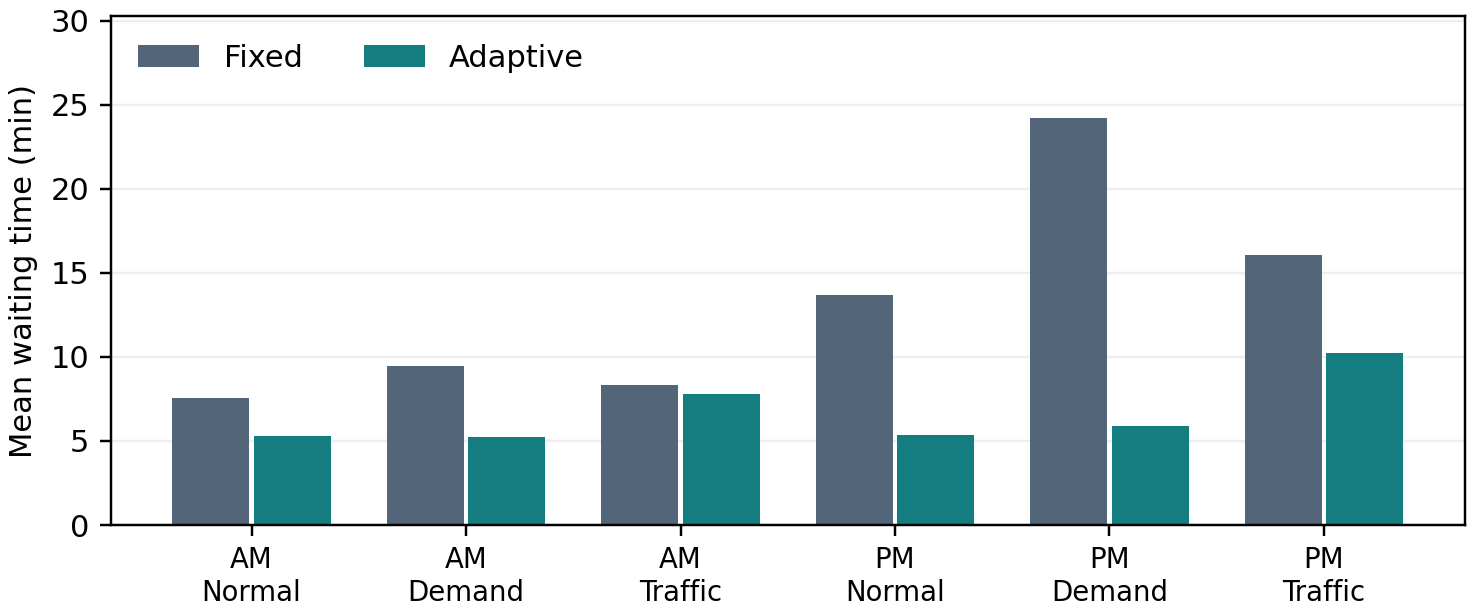
\includegraphics[width=\columnwidth]{waiting.png}\caption{Mean waiting time across the six scenarios.}\end{figure}
\begin{figure}[h]\centering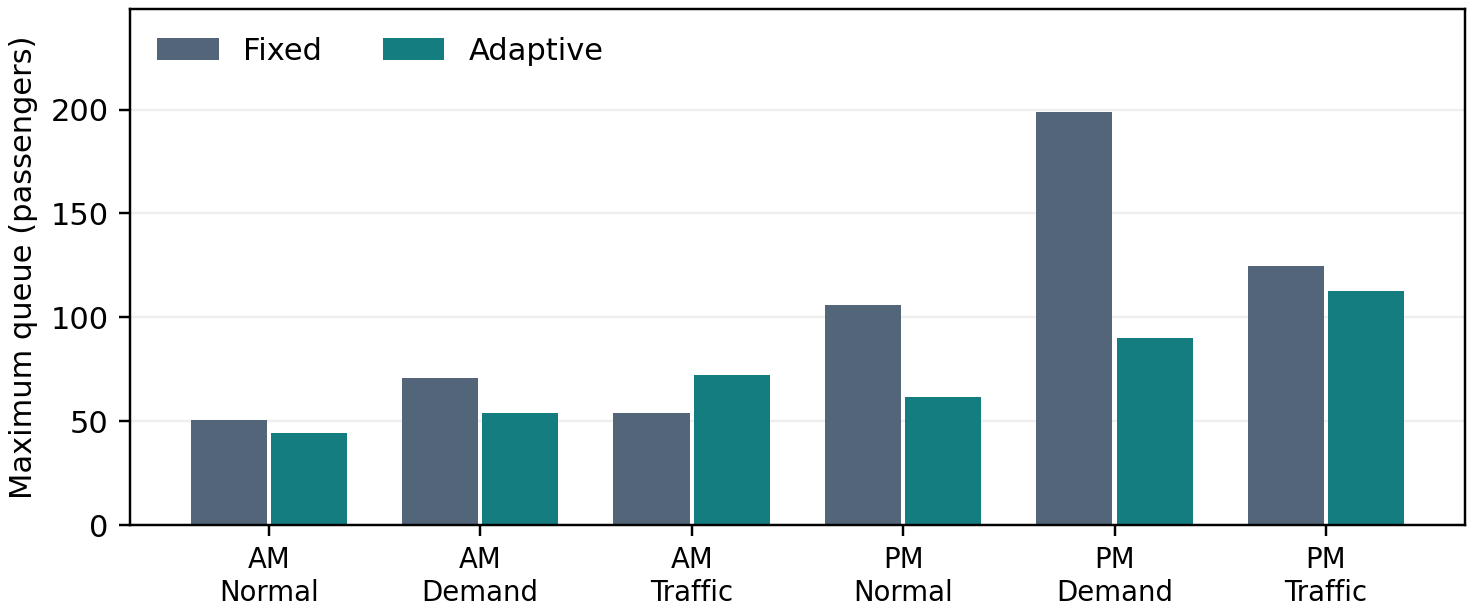
\includegraphics[width=\columnwidth]{queue.png}\caption{Maximum combined passenger queue.}\end{figure}
\begin{figure}[h]\centering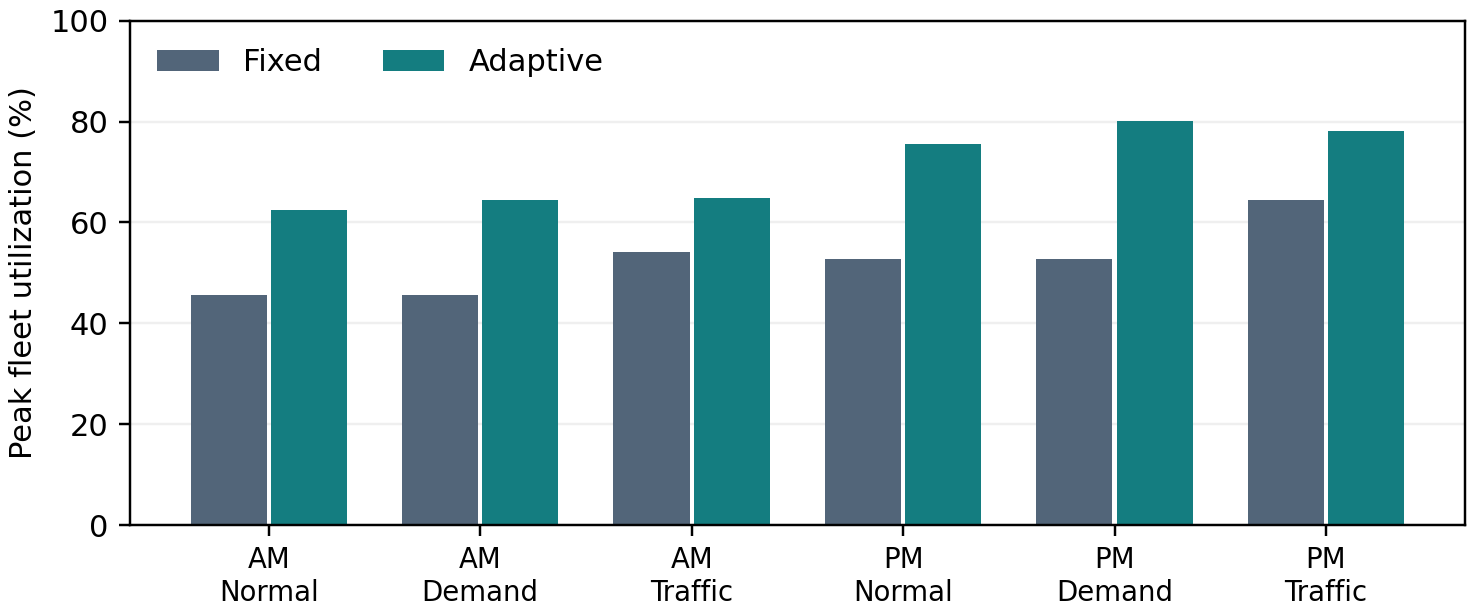
\includegraphics[width=\columnwidth]{utilization.png}\caption{Time-based fleet utilization during peak periods.}\end{figure}
\subsection{Normal peak operation}
In the morning, adaptive scheduling reduces mean wait from 7.54 to 5.27 minutes (30.2\%). In the afternoon, it decreases from 13.69 to 5.35 minutes (60.9\%). Afternoon backlog drops from 105.3 to 25.2 passengers on average, and utilization increases by 22.9 percentage points. This indicates that the fixed timetable leaves buses unused even when passenger demand is high.
\subsection{High demand and traffic delays}
Under increased afternoon demand, the fixed timetable produces a mean wait of 24.21 minutes and a maximum combined queue of approximately 199 passengers. Adaptive dispatch cuts mean wait to 5.91 minutes and maximum queue to about 90 passengers. Under afternoon traffic delays, mean wait declines from 16.08 to 10.21 minutes, but congestion remains. Morning traffic delays are a counterexample: adaptive dispatch slightly reduces mean wait, yet maximum queue increases from 53.8 to 72.3. The heuristic is not uniformly superior on every metric.
\subsection{Efficiency trade-off}
Adaptive dispatch increases normal afternoon trips from 14.9 to 18.5 and reduces average seat load from 77.2\% to 62.3\%. More frequent departures improve service at the cost of potentially higher fuel use and driver workload. These costs are not quantified by the available model. The objective should be a balance of waiting time, safety and vehicle efficiency, not simply the highest utilization percentage.
\section{Recommendations and limitations}
\begin{enumerate}
\item Collect timestamped passenger arrivals, boarding counts, actual headways, vehicle capacities, GPS trip durations, route assignments and driver availability at both terminals.
\item Pilot the threshold policy with existing buses, digital queue counts and a dispatcher display showing queue length, oldest wait and vehicle status. Keep a hard capacity limit and FCFS boarding.
\item Calibrate the load threshold and wait trigger against observed data. During congestion, test a higher minimum load or reserve policy to avoid exhausting the fleet too early. Compare wait, queue, fuel use and service fairness before selecting parameters.
\item Use GPS-based estimated return times and route-compatible vehicle assignment. Include driver breaks, distinct origin/destination routes, physical boarding times and travel-time variation in a subsequent model.
\item Monitor P95 and backlog in addition to the mean. Retain manual dispatcher intervention and fixed minimum service for low-demand routes.
\end{enumerate}
The model assumes a shared pool that can reposition within trip time; real route constraints may reduce flexibility. It does not model individual destinations, actual road geometry, abandonment, continuous all-day operation, vehicle breakdowns or measured operating costs. The assumed fleet and demand should be replaced with verified data before operational use. The results are illustrative and no claim of global optimality is made.
\section{Conclusion}
The DES demonstrates how queue-aware dispatch can improve passenger service with the same fleet under assumed peak conditions. The largest modeled benefit occurs in high-demand afternoons, while traffic delays expose remaining capacity constraints. A calibrated, route-aware pilot is recommended rather than immediate fleet expansion.
\begin{thebibliography}{1}
\bibitem{brief} Department of Software Engineering, MUET, ``Simulation \& Modelling: Problem Based Learning (PBL), Batch 22SW II \& III,'' assignment brief, pp. 1--2.
\end{thebibliography}
\end{document}
